\documentclass[12pt]{article}
\usepackage[french]{babel}
\usepackage[utf8]{inputenc}
\usepackage{amsmath}
\usepackage{graphicx}
\graphicspath{{Images/}}
\usepackage[colorinlistoftodos]{todonotes}
\usepackage{hyperref}
%\usepackage{apple_emoji}
\usepackage{tikz}
\usepackage{subcaption}

\usepackage{parskip}
\setlength{\parindent}{1cm}
\usepackage{indentfirst}

\usepackage{enumitem}
\setitemize{noitemsep,topsep=0pt,parsep=0pt,partopsep=0pt}

\begin{document}
\begin{titlepage}
\newcommand{\HRule}{\rule{\linewidth}{0.1mm}} 
\center % Center everything on the page
 
%---------------------------------------------------------------------------------
%	HEADING SECTIONS (Enter the Homework/assignment No., only)
%---------------------------------------------------------------------------------
\textsc{\Large Linux/GNU}\\[0.3cm] % heading ourse Number
\textsc{\Large Pertinance d'une évolution de Buildroot à Yocto }\\[0.3cm] % heading course name

%---------------------------------------------------------------------------------
%	TITLE SECTION (Replace 'TITLE' with the Homework/assignment Name/title)
%---------------------------------------------------------------------------------

\HRule \\[0.4cm]
{ \huge \bfseries YOCTO}\\[0.1cm] % Title of your Homework/assignment
\HRule \\[1.5cm]
 
%---------------------------------------------------------------------------------
%	AUTHOR SECTION (EDIT THE NAME and T.NO., only)
%---------------------------------------------------------------------------------

\begin{minipage}{0.4\textwidth}
\begin{flushleft} \large
Colin \textsc{Baumgard}\\  % Enter Your name and T.No.
\end{flushleft}

\end{minipage}
\begin{minipage}{0.4\textwidth}
    \begin{flushleft} \large
        Paul-Antoine \textsc{Le Tolguenec}\\  % Enter Your name and T.No.
        \end{flushleft}

      
\end{minipage}\\[1cm]
{\large \today}\\[1cm] % Date, change the \today to a set date if you want to be precise

\includegraphics{ENSTA1246-524.png}% \\[0.5cm] % 
\vfill % Fill the rest of the page with white-space

\end{titlepage}
\include{GradingRubric}
\tableofcontents          % Required
\listoffigures
\listoftables
\newpage


% Chapters including
\section{Introduction}
\paragraph{}
ecris ici

\textbf{Repo GitHub}

\url{https://github.com/Paul-antoineLeTolguenec/Linux-GNU.git}

\newpage


\section{Buildroot}
\paragraph{}
Buildroot est un framework permettant de compiler un linux embarqué. Pendant longtemps buildroot a été la référence. Il propose, via un outil graphique, de paramétrer son système en fonction de ses besoins.

\begin{figure}[!h]
    \center
    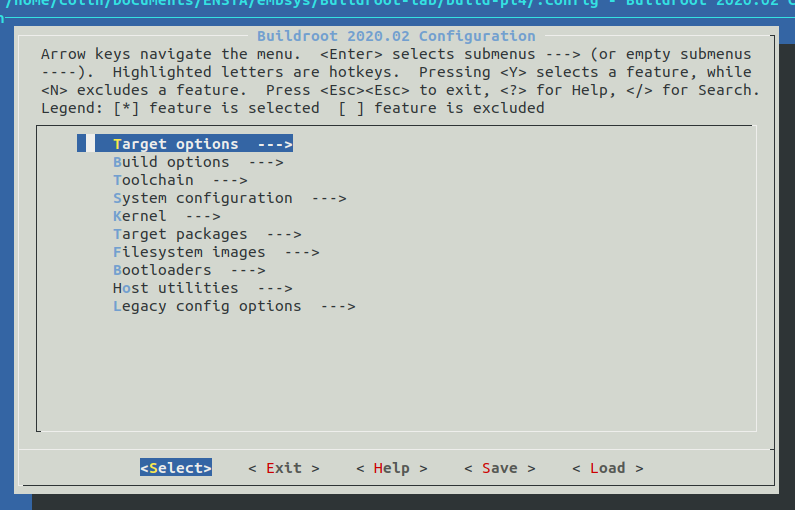
\includegraphics[width=10cm]{Images/menuconfig.png}
    \caption{Menu obtenu par ma commande \$make menuconfig}
\end{figure}

\paragraph{}
L'ajout de code métier ou de packages non présents dans le menu est bien sûr possible.
Cependant avec la diversification des applications et les temps de développements courts, les développeurs ont de plus en plus recours à des modules externes. Et c'est là que Buildroot montre ses limites. Chaque mise à jour implique une recompilation de tout le système, entraînant une certaine lourdeur. Il est à noter que Buildroot utilise l'outil GNU-Make, et n'utilise pas de fait des threads (il utilise bien entendu tous les coeurs du processeur à disposition), fonctionnalité dont est pourvu Yocto qui peut simultanément télécharger, configurer et compiler, optimisant ainsi le processus.





\section{Yocto: pour qui ? pourquoi?}

Pour construire son OS aujourd'hui, il existe de nombreux outils. Un outils (ou plutôt ensemble d'outils) très utilisé est buildroot. Mais il en exeiste plein d'autre.
Dans le monde de l'industrie le projet Yocto est de plus en plus présent et nous allons voir pourquoi.
\subsection{Les outils disponibles pour construire son OS aujourd'hui}
\paragraph{}

Comme nous l'avons dit, les outils permettant la création d'OS sont multiples.
Voici une synthèse des principaux :
\paragraph{}
Do It Yourself : limité aux cas simples
\begin{itemize} 

\item Avantage = maîtrise totale

\item Inconvénient = il faut tout faire
\end{itemize} 

\paragraph{}
Buildroot : simple mais fonctionnellement moins
riches que les autres
\begin{itemize} 

\item Adapté aux applications enfouies, pas très riches

\item Difficile de travailler en différentiel : régénération complète du
File System, pas de gestion de paquets

\item Basé sur des Makefiles
\end{itemize} 

\paragraph{}
Scratchbox : riche mais obsolète

\paragraph{}
LTIB : outil utilisé par Freescale, mais changement en
cours au profit du Yocto Project

\begin{itemize} 

\item Versions logicielles datées (host + target)

\end{itemize} 



\paragraph{}
OpenEmbedded : Ancêtre commun issu du projet Open Zaurus, toujours actif.
\begin{itemize} 

\item Base de distributions variées

\end{itemize} 
\paragraph{}
Et il en existe encore bien d'autre. Mais alors avec cette forte diversité pourquoi choisir YOCTO ?
Les avantages sont multiples bien sûr, mais le plus important est son côté modulable.
Aussi, ce projet permet de mettre en place de manière industrielle des outils de création de distribution Linux embarqué. C'est donc un projet oprmisé pour le monde de l'industrie.
En effet, du fait de l'évolution des compasants d'un système il faut avoir une certaine flexibilité sur l'OS que l'on conçoit. Yocto permet cette flexibilité.
De plus, le projet Yocto est sous l'égide de la Linux Foundation ce qui permet une certaine garantie de fonctionnement.
On voit donc un peu plus pourquoi Yocto est apprécié des industriels.
Mais comme nous l'avons vu ce projet ce distingue notamment de par sa fléxibilité.
Nous allons maintenant expliquer comment cette flexibilité est permise.





\subsection{Yocto : un fonctionnement plus flexible}
\begin{figure}[ht!]

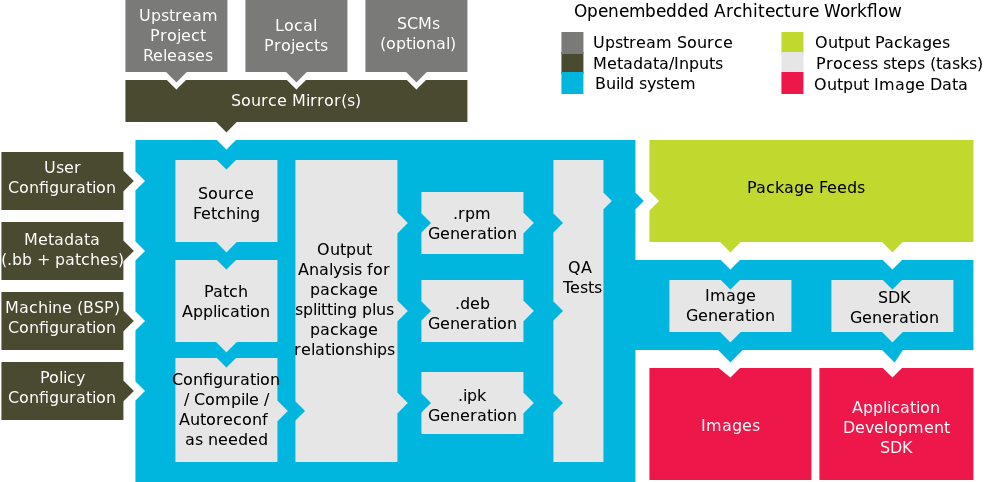
\includegraphics[width=\linewidth]{yocto.png} % Figure image 

\caption{crédit: Yocto project} % Figure caption 


\label{Project Yocto} % Label for referencing with \ref{bear} 
\end{figure}


\paragraph{}
Yocto intègre des parties développées conjointement pour OpenEmbedded, notamment BitBake, OpenEmbedded-Core et d'autres métadonnées. 
Les éléments développés dans le cadre du projet, appelés "meta-yocto" et "meta-yocto-bsp", comprennent l'intégration des éclipses. 
Ensemble, ils améliorent les outils d'OpenEmbedded, cette plateforme de référence pour la construction de systèmes avancés embarqués dans les HW est connue 
sous le nom de Poky.

Pour développer des logiciels, nous avons besoin d'une chaîne d'outils (croisés) : les fichiers sources et les instructions sur la façon de les compiler. 
C'est suffisant pour une source. 
Pour plus de composants et de dépendances dans la compilation et le temps d'exécution, il faut augmenter la complexité et des étapes supplémentaires. 
Bitbake est un agent ayant la capacité d'interpréter et d'exécuter les recettes d'amélioration, il calcule la chaîne des tâches nécessaires pour développer l'objectif défini et exécuté. 



\section{Discussions et Conclusion}

\subsubsection{Yocto ou Buildroot, comment choisir ?}
\paragraph{}
Yocto est donc très adapté pour une image nécessitant une multitude de dépendances externes, pour un développement court et focalisé sur les fonctionnalités propres du produit, avec une gamme de produits proposant des fonctionnalités légèrement différentes. Yocto permet de factoriser le développement et de rendre modulable l'OS embarqué.  Buildroot est, quant à lui, plus adapté à des projets plus modestes, où la mise à jour est moins fréquente. Buildroot crée des OS statiques, adaptés aux outils plus bas niveau, peut être moins évolués, se focalisants sur la robustesse. Buildroot est également plus simple à prendre en main, ce qui est un atout non négligeable. Il sera en revanche moins adapté au travail en groupe. 


\begin{figure}[ht!] 
\begin{center}
    

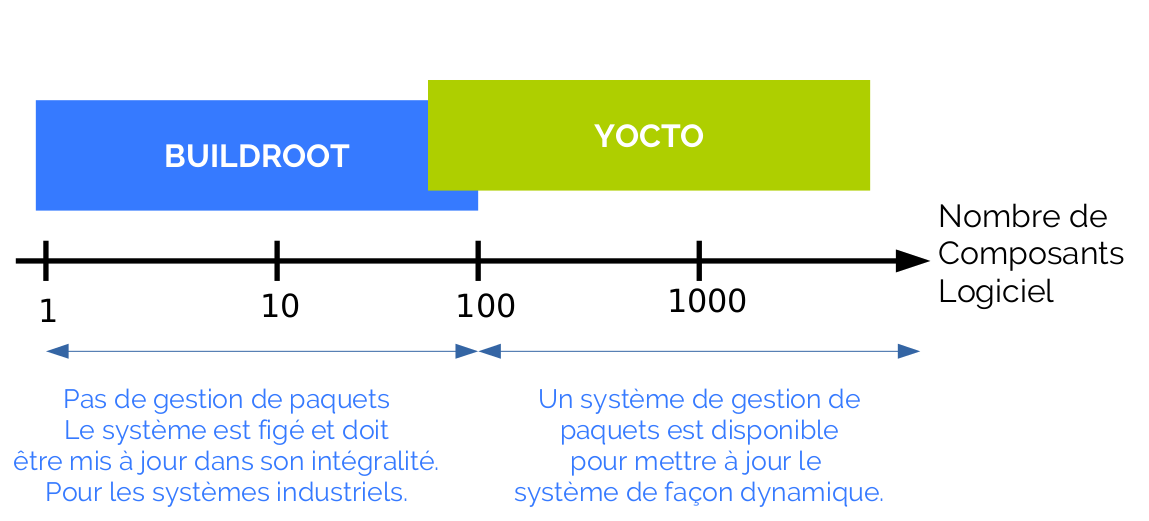
\includegraphics[width=13cm]{Images/yocto comp log.png} % Figure image 

\caption{crédit: Yocto project} % Figure caption 

\end{center}
\label{Project Yocto} % Label for referencing with \ref{bear} 
\end{figure}

On peut donc résumer : 
Le projet
\begin{itemize}

\item comporte une gamme de produit - Yocto facilitera la factorisation du développement
\item comporte de nombreux modules externe - Yocto
\item repose sur des ajouts de fonctionnalité fréquentes - Yocto
\item est un système figé, un code métier peu évolutif et peu de composants externe - Buildroot fera très bien l'affaire
\end{itemize}

Tout ce que peut faire Buildroot, Yocto en est également capable. Le passage de Buildroot à Yocto est pertinent si le projet est important, qu'il doit être porté sur différentes plateformes et qu'il nécessite de nombreuses composantes de la communauté. Si la composante centrale du projet n'est pas logiciel, que tout repose sur le code métier, avec un cycle de développement long, Buildroot est adapté et une évolution n'est pas forcément pertinente.


\bibliographystyle{unsrt}
\bibliography{./Chapters/Bibliographie}

\end{document}
